\section{Generación de energía}
\subsection{Enunciado 12.5}
\paragraph{} Varias centrales eléctricas se comprometen a cumplir las siguientes demandas de carga de electricidad durante un día:\\
\begin{center}
\begin{tabular}{cc}
\hline 
12 pm a 6 am & 15000 MW \\  
6 am a 9 am & 30000 MW \\  
9 am a 3 pm & 25000 MW \\  
3 pm a 6 pm & 40000 MW \\  
6 pm a 12 pm & 27000 MW \\ 
\hline 
\end{tabular} 
\end{center}

\paragraph{} Hay tres tipos de unidades generadoras disponibles: 12 de tipo 1, 10 de tipo 2 y cinco de tipo 3. Cada generador tiene que funcionar entre un nivel mínimo y un nivel máximo. Hay un costo por hora de funcionamiento de cada generador al nivel mínimo. Además, hay un costo adicional por hora por cada megavatio en el que se opera una unidad por encima del nivel mínimo. Iniciar un generador también implica un costo. Toda esta información se da en la tabla 12.6 (con costos en \pounds).
\begin{center}
\begin{tabular}{cccccc}
\hline 
 & Nivel & Nivel & Costo por  & Costo por hora & Costo \\ 
 & Minimo & Maximo & hora como & por megavatio &  \\ 
 &  &  & minimo & $>$ minimo &  \\ 
\hline 
Type 1 & 850 MW & 2000 MW & 1000 & 2 & 2000 \\ 
Type 2 & 1250 MW & 1750 MW & 2600 & 1.30 & 1000 \\ 
Type 3 & 1500 MW & 4000 MW & 3000 & 3 & 500 \\ 
\hline 
\end{tabular} 
\end{center}

\paragraph{} Además de cumplir con las demandas de carga estimadas, debe haber suficientes generadores trabajando en todo momento para que sea posible cumplir con un aumento en la carga de hasta 15\%. Este aumento tendría que lograrse ajustando la producción de los generadores que ya operan dentro de sus límites permitidos.

\paragraph{} ¿Qué generadores deberían estar trabajando en qué períodos del día para minimizar el costo total?

\paragraph{} ¿Cuál es el costo marginal de producción de electricidad en cada período del día?; es decir, ¿qué aranceles deberían cobrarse?

\paragraph{} ¿Cuál sería el ahorro de reducir la garantía de reserva del aumento en la carga de hasta el 15\%? es decir, ¿cuánto cuesta esta garantía de reserva de suministro?


\subsection{Modelo 12.5}
$\begin{array}{l}
T12a6_{i}:\mbox{\# de generadores tipo i usados desde 12 pm a 6 am}\\
C12a6_{i}:\mbox{\# de energia proporcionada por generador tipo i desde 12 pm a 6 am}\\
F12a6_{i}:\mbox{\# de energia con costo adicional generador tipo i desde 12 pm a 6 am}\\
P12a6_{i}:\mbox{costo total generador tipo i desde 12 pm a 6 am}\\
PF12a6:\mbox{costo total 12 pm a 6 am}\\
T6a9_{i}:\mbox{\# de generadores tipo i usados desde 6 am a 9 am}\\
C6a9_{i}:\mbox{\# de energia proporcionada por generador tipo i desde 6 am a 9 am}\\
F6a9_{i}:\mbox{\# de energia con costo adicional generador tipo i desde 6 am a 9 am}\\
P6a9_{i}:\mbox{costo total generador tipo i desde 6 am a 9 am}\\
PF6a9:\mbox{costo total 6 am a 9 am}\\
T9a3_{i}:\mbox{\# de generadores tipo i usados desde 9 am a 3 pm}\\
C9a3_{i}:\mbox{\# de energia proporcionada por generador tipo i desde 9 am a 3 pm}\\
F9a3_{i}:\mbox{\# de energia con costo adicional generador tipo i desde 9 am a 3 pm}\\
P9a3_{i}:\mbox{costo total generador tipo i desde 9 am a 3 pm}\\
PF9a3:\mbox{costo total 9 am a 3 pm}\\
T3a6_{i}:\mbox{\# de generadores tipo i usados desde 3 pm a 6 pm}\\
C3a6_{i}:\mbox{\# de energia proporcionada por generador tipo i desde 3 pm a 6 pm}\\
F3a6_{i}:\mbox{\# de energia con costo adicional generador tipo i desde 3 pm a 6 pm}\\
P3a6_{i}:\mbox{costo total generador tipo i desde 3 pm a 6 pm}\\
PF3a6:\mbox{costo total 3 pm a 6 pm}\\
T6a12_{i}:\mbox{\# de generadores tipo i usados desde 6 pm a 12 pm}\\
C6a12_{i}:\mbox{\# de energia proporcionada por generador tipo i desde 6 pm a 12 pm}\\
F6a12_{i}:\mbox{\# de energia con costo adicional generador tipo i desde 6 pm a 12 pm}\\
P6a12_{i}:\mbox{costo total generador tipo i desde 6 pm a 12 pm}\\
PF6a12:\mbox{costo total 6 pm a 12 pm}\\
\mbox{donde} \;\;\;\;\;\; i=1,2,3   
\end{array}$
\\
\\
$$ \mbox{min } PF12a6 + PF6a9 + PF9a3 + PF3a6 + PF6a12 $$
\\ 
\\  
s.a\\
\begin{equation}
T12a6_{1} \leq 12
\end{equation}
\begin{equation}
T6a9_{1} \leq 12
\end{equation}
\begin{equation}
T9a3_{1} \leq 12
\end{equation}
\begin{equation}
T3a6_{1} \leq 12
\end{equation}
\begin{equation}
T6a12_{1} \leq 12 
\end{equation}
\begin{equation}
T12a6_{2} \leq 10
\end{equation}
\begin{equation}
T6a9_{2} \leq 10
\end{equation}
\begin{equation}
T9a3_{2} \leq 10
\end{equation}
\begin{equation}
T3a6_{2} \leq 10
\end{equation}
\begin{equation}
T6a12_{2} \leq 10 
\end{equation}
\begin{equation}
T12a6_{3} \leq 5
\end{equation}
\begin{equation}
T6a9_{3} \leq 5
\end{equation}
\begin{equation}
T9a3_{3} \leq 5
\end{equation}
\begin{equation}
T3a6_{3} \leq 5
\end{equation}
\begin{equation}
T6a12_{3} \leq 5 
\end{equation}
%%%%%%%%%%%%%%%%%%%%%%%%%%%%%%%%Energia por horario 12 a 6
%la cantidad de energia debe estar en entre cantidad por el minimo y la cantidad por el maximo
%TIPO 1
\begin{equation}
C12a6_{1} \geq 850 T12a6_{1}
\end{equation}
\begin{equation}
C12a6_{1} \leq 2000 T12a6_{1}
\end{equation}
\begin{equation}
E12a6_{1} = C12a6_{1} - 850 T12a6_{1}
\end{equation}
\begin{equation}
P12a6_{1} = 2000 + 2 \; E12a6_{1} + 6 \; 1000 \; T12a6_{1}
\end{equation}
%TIPO 2
\begin{equation}
C12a6_{2} \geq 1250 T12a6_{2}
\end{equation}
\begin{equation}
C12a6_{2} \leq 1750 T12a6_{2}
\end{equation}
\begin{equation}
E12a6_{2} = C12a6_{2} - 1250 T12a6_{3}
\end{equation}
\begin{equation}
P12a6_{2} = 1000 + 1.30 \; E12a6_{2} + 6 \; 2600 \; T12a6_{3}
\end{equation}
%TIPO 3
\begin{equation}
C12a6_{3} \geq 1500 T12a6_{3}
\end{equation}
\begin{equation}
C12a6_{3} \leq 4000 T12a6_{3}
\end{equation}
\begin{equation}
E12a6_{3} = C12a6_{3} - 1500 T12a6_{3}
\end{equation}
\begin{equation}
P12a6_{3} = 500 + 3 \; E12a6_{3} + 6 \; 3000 \; T12a6_{3}
\end{equation}
\begin{equation}
PF12a6 = P12a6_{1} + P12a6_{2} + P12a6_{3} 
\end{equation}
%%%%%%%%%%%%%%%%%%%%%%%%%%%%%%%%Energia por horario 6 a 9
%la cantidad de energia debe estar en entre cantidad por el minimo y la cantidad por el maximo
%TIPO 1
\begin{equation}
C6a9_{1} \geq 850 T6a9_{1}
\end{equation}
\begin{equation}
C6a9_{1} \leq 2000 T6a9_{1}
\end{equation}
\begin{equation}
E6a9_{1} = C6a9_{1} - 850 T6a9_{1}
\end{equation}
\begin{equation}
P6a9_{1} = 2000 + 2 E6a9_{1} + 3 \; 1000 \; T6a9_{1}
\end{equation}
%TIPO 2
\begin{equation}
C6a9_{2} \geq 1250 T6a9_{2}
\end{equation}
\begin{equation}
C6a9_{2} \leq 1750 T6a9_{2}
\end{equation}
\begin{equation}
E6a9_{2} = C6a9_{2} - 1250 T6a9_{2}
\end{equation}
\begin{equation}
P6a9_{2} = 1000 + 1.30 E6a9_{2} + 3 \; 2600  \;T6a9_{2}
\end{equation}
%TIPO 3
\begin{equation}
C6a9_{3} \geq 1500 T6a9_{3}
\end{equation}
\begin{equation}
C6a9_{3} \leq 4000 T6a9_{3}
\end{equation}
\begin{equation}
E6a9_{3} = C6a9_{3} - 1500 T6a9_{3}
\end{equation}
\begin{equation}
P6a9_{3} = 500+ 3 \; E6a9_{3} + 3 \; 3000 \; T6a9_{3}
\end{equation}
\begin{equation}
PF6a9 = P6a9_{1} + P6a9_{2} + P6a9_{3}
\end{equation}
%%%%%%%%%%%%%%%%%%%%%%%%%%%%%%%%Energia por horario 9 a 3
%la cantidad de energia debe estar en entre cantidad por el minimo y la cantidad por el maximo
%TIPO 1
\begin{equation}
C9a3_{1} \geq 850 T9a3_{1}
\end{equation}
\begin{equation}
C9a3_{1} \leq 2000 T9a3_{1}
\end{equation}
\begin{equation}
E9a3_{1} = C9a3_{1} - 850 T9a3_{1}
\end{equation}
\begin{equation}
P9a3_{1} = 2000 + 2 \; E9a3_{1} + 6 \; 1000 \; T9a3_{1}
\end{equation}
%TIPO 2
\begin{equation}
C9a3_{2} \geq 1250 T9a3_{2}
\end{equation}
\begin{equation}
C9a3_{2} \leq 1750 T9a3_{2}
\end{equation}
\begin{equation}
E9a3_{2} = C9a3_{2} - 1250 T9a3_{2}
\end{equation}
\begin{equation}
P9a3_{2} = 1000 + 1.30 \; E9a3_{2} + 6 \; 2600 \; T9a3_{2}
\end{equation}
%TIPO 3
\begin{equation}
C9a3_{3} \geq 1500 T9a3_{3}
\end{equation}
\begin{equation}
C9a3_{3} \leq 4000 T9a3_{3}
\end{equation}
\begin{equation}
E9a3_{3} = C9a3_{3} - 1500 T9a3_{3}
\end{equation}
\begin{equation}
P9a3_{3} = 500 + 3 \; E9a3_{3} + 6 \; 3000 \; T9a3_{3}
\end{equation}
\begin{equation}
PF9a3 = P9a3_{1} + P9a3_{2} + P9a3_{3}
\end{equation}
%%%%%%%%%%%%%%%%%%%%%%%%%%%%%%%%Energia por horario 3a6
%la cantidad de energia debe estar en entre cantidad por el minimo y la cantidad por el maximo
%TIPO 1
\begin{equation}
C3a6_{1} \geq 850 T3a6_{1}
\end{equation}
\begin{equation}
C3a6_{1} \leq 2000 T3a6_{1}
\end{equation}
\begin{equation}
E3a6_{1} = C3a6_{1} - 850 T3a6_{1}
\end{equation}
\begin{equation}
P3a6_{1} = 2000 + 2 \; E3a6_{1} + 3 \; 1000 \; T3a6_{1}
\end{equation}
%TIPO 2
\begin{equation}
C3a6_{2} \geq 1250 T3a6_{2}
\end{equation}
\begin{equation}
C3a6_{2} \leq 1750 T3a6_{2}
\end{equation}
\begin{equation}
E3a6_{2} = C3a6_{2} - 1250 T3a6_{2}
\end{equation}
\begin{equation}
P3a6_{2} = 1000 + 1.30 \; E3a6_{2} + 3 \; 2600 \; T3a6_{2}
\end{equation}
%TIPO 3
\begin{equation}
C3a6_{3} \geq 1500 T3a6_{3}
\end{equation}
\begin{equation}
C3a6_{3} \leq 4000 T3a6_{3}
\end{equation}
\begin{equation}
E3a6_{3} = C3a6_{3} - 1500 T3a6_{3}
\end{equation}
\begin{equation}
P3a6_{3} = 500 + 3 \; E3a6_{3} + 3 \; 3000 \; T3a6_{3}
\end{equation}
\begin{equation}
PF3a6 = P3a6_{1} + P3a6_{2} + P3a6_{3}
\end{equation}
%%%%%%%%%%%%%%%%%%%%%%%%%%%%%%%%Energia por horario 6 a 12
%la cantidad de energia debe estar en entre cantidad por el minimo y la cantidad por el maximo
%TIPO 1
\begin{equation}
C6a12_{1} \geq 850 T6a12_{1}
\end{equation}
\begin{equation}
C6a12_{1} \leq 2000 T6a12_{1}
\end{equation}
\begin{equation}
E6a12_{1} = C6a12_{1} - 850 T6a12_{1}
\end{equation}
\begin{equation}
P6a12_{1} = 2000 + 2 \; E6a12_{1} + 6 \; 1000 \; T6a12_{1}
\end{equation}
%TIPO 2
\begin{equation}
C6a12_{2} \geq 1250 T6a12_{2}
\end{equation}
\begin{equation}
C6a12_{2} \leq 1750 T6a12_{2}
\end{equation}
\begin{equation}
E6a12_{2} = C6a12_{2} - 1250 T6a12_{2}
\end{equation}
\begin{equation}
P6a12_{2} = 1000 + 1.30 \; E6a12_{2} + 6 \; 2600 \; T6a12_{2}
\end{equation}
%TIPO 3
\begin{equation}
C6a12_{3} \geq 1500 T6a12_{3}
\end{equation}
\begin{equation}
C6a12_{3} \leq 4000 T6a12_{3}
\end{equation}
\begin{equation}
E6a12_{3} = C6a12_{3} - 1500 T6a12_{3}
\end{equation}
\begin{equation}
P6a12_{3} = 500 + 3 \; E6a12_{3} + 6 \; 3000 \; T6a12_{3}
\end{equation}
\begin{equation}
PF6a12 = P6a12_{1} + P6a12_{2} + P6a12_{3}
\end{equation}
%%%%%%%%%%%%%%%%%%%%%%%%%%%%%%%%%%%%%%%%%%%%
% Se deben cumplir con los requerimientos por horarios
%\begin{equation}
%C12a6_{1} + C12a6_{2} + C12a6_{3}  \geq 15000
%\end{equation}
\begin{equation}
C12a6_{1} + C12a6_{2} + C12a6_{3} \geq 17250
\end{equation}
%\begin{equation}
%C6a9_{1} + C6a9_{2} + C6a9_{3} \geq 30000
%\end{equation}
\begin{equation}
C6a9_{1} + C6a9_{2} + C6a9_{3} \geq 34500
\end{equation}
%\begin{equation}
%C9a3_{1} + C9a3_{2} + C9a3_{3} \geq 25000
%\end{equation}
\begin{equation}
C9a3_{1} + C9a3_{2} + C9a3_{3} \geq 28750
\end{equation}
%\begin{equation}
%C3a6_{1} + C3a6_{2} + C3a6_{3} \geq 40000
%\end{equation}
\begin{equation}
C3a6_{1} + C3a6_{2} + C3a6_{3} \geq 46000
\end{equation}
%\begin{equation}
%C6a12_{1} + C6a12_{2} + C6a12_{3} \geq 27000
%\end{equation}
\begin{equation}
C6a12_{1} + C6a12_{2} + C6a12_{3} \geq 31050
\end{equation}
\subsection{Modelo CPLEX 12-15}
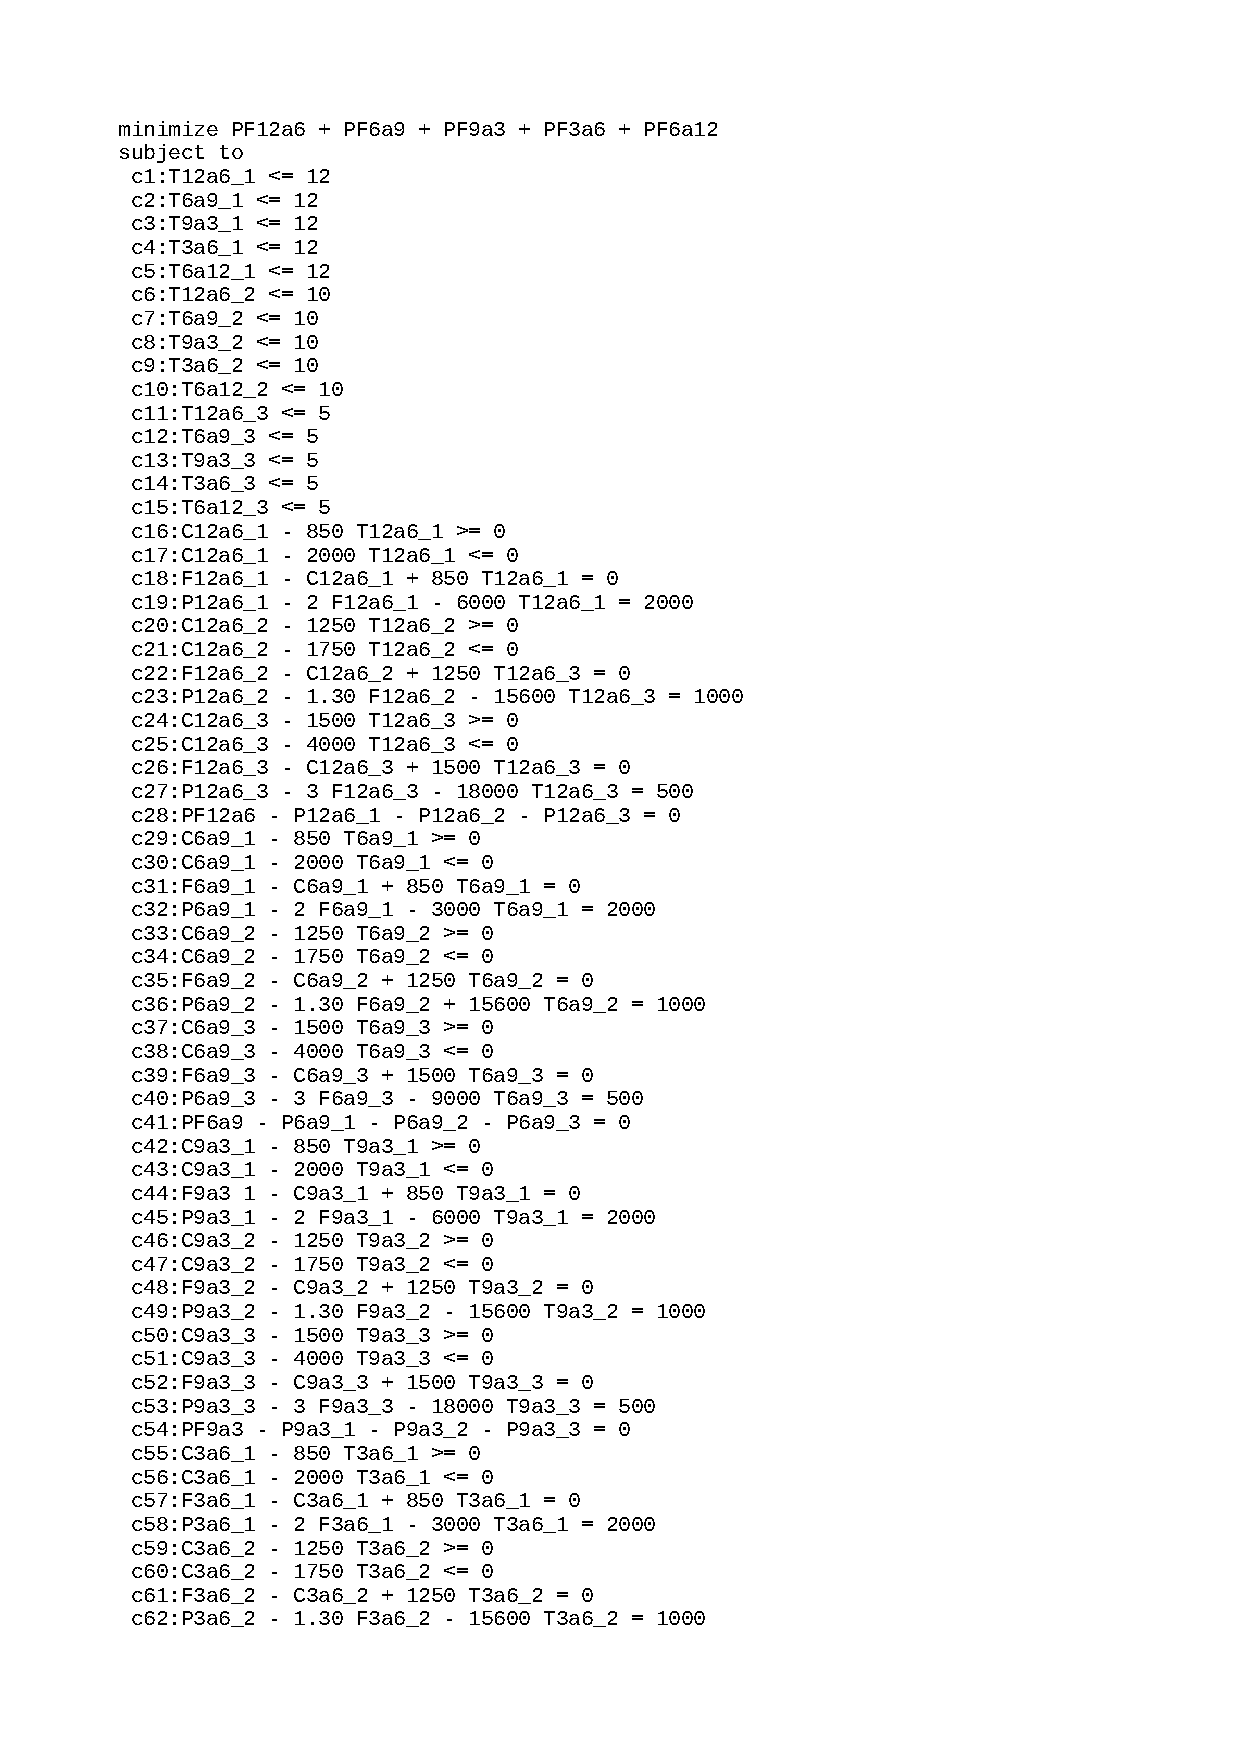
\includepdf[pages=1-2]{modelos/centralElectrica12-15}
\subsection{Solucion en CPLEX}

\paragraph{} ¿Qué generadores deberían estar trabajando en qué períodos del día para minimizar el costo total?
\begin{figure}[!h]
    \centering
    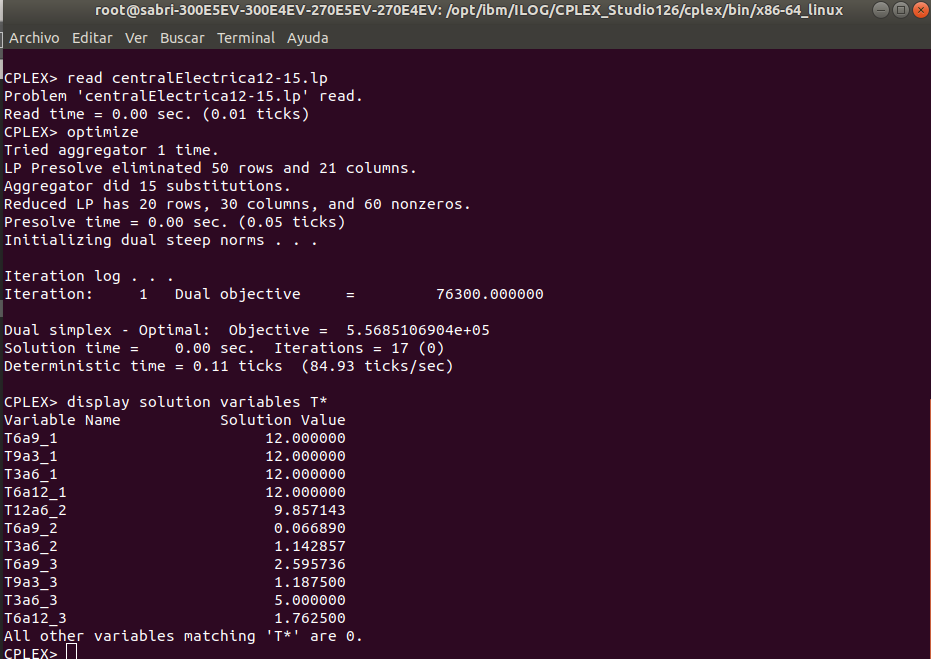
\includegraphics[scale=0.35]{modelos/SolutionCentralElectrica12-15Generadores.png}
    \caption{SolucionCentraElectricaGeneradores}
\end{figure}

\paragraph{} ¿Cuál es el costo marginal de producción de electricidad en cada período del día?; es decir, ¿qué aranceles deberían cobrarse?
\begin{figure}[!h]
    \centering
    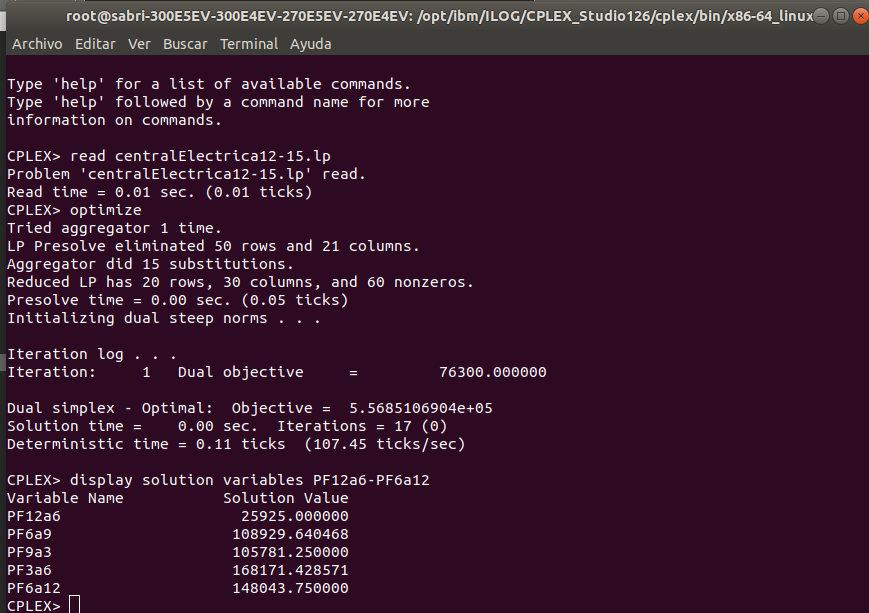
\includegraphics[scale=0.35]{modelos/SolutionCentralElectrica12-15PrecioPorRango.png}
    \caption{SolucionCentraElectricaGeneradores}
\end{figure}

\paragraph{} ¿Cuál sería el ahorro de reducir la garantía de reserva del aumento en la carga de hasta el 15\%? es decir, ¿cuánto cuesta esta garantía de reserva de suministro?\\
Modificamos estas restricciones:
\begin{equation}
C12a6_{1} + C12a6_{2} + C12a6_{3} \geq 17250
\end{equation}
\begin{equation}
C6a9_{1} + C6a9_{2} + C6a9_{3} \geq 34500
\end{equation}
\begin{equation}
C9a3_{1} + C9a3_{2} + C9a3_{3} \geq 28750
\end{equation}
\begin{equation}
C3a6_{1} + C3a6_{2} + C3a6_{3} \geq 46000
\end{equation}
\begin{equation}
C6a12_{1} + C6a12_{2} + C6a12_{3} \geq 31050
\end{equation}
\\ 
 por

\begin{equation}
C12a6_{1} + C12a6_{2} + C12a6_{3} \geq 15000
\end{equation}
\begin{equation}
C6a9_{1} + C6a9_{2} + C6a9_{3} \geq 30000
\end{equation}
\begin{equation}
C9a3_{1} + C9a3_{2} + C9a3_{3} \geq 25000
\end{equation}
\begin{equation}
C3a6_{1} + C3a6_{2} + C3a6_{3} \geq 40000
\end{equation}
\begin{equation}
C6a12_{1} + C6a12_{2} + C6a12_{3} \geq 27000
\end{equation}

\begin{figure}[!h]
    \centering
    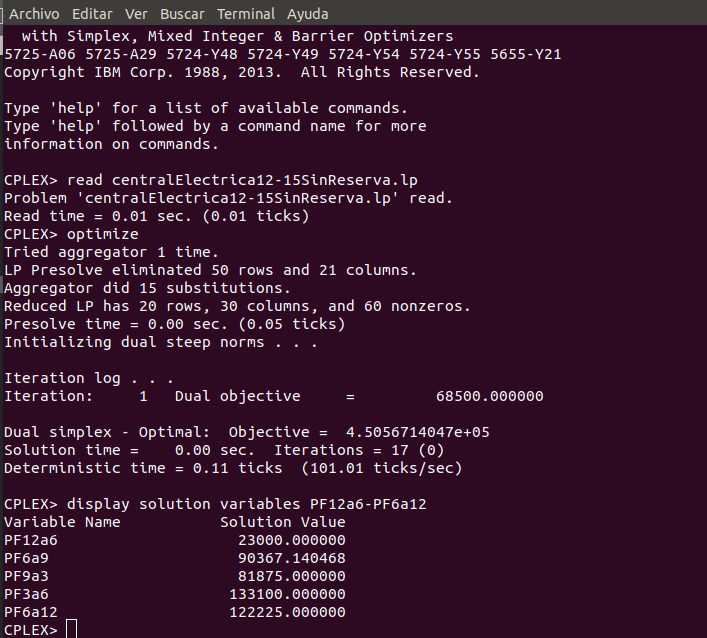
\includegraphics[scale=0.35]{modelos/SolutionCentralElectrica12-15PrecioPorRangoSinReserva.png}
    \caption{SolucionCentraElectricaGeneradores}
\end{figure}

\section{Energía hidroeléctrica}
\subsection{Enunciado 12.6}
\paragraph{} Esta es una extensión del problema de generación de energía. Además de los generadores térmicos, un depósito alimenta dos hidrogeneradores: en el tipo A y uno de tipo B. Cuando un hidrogenerador está funcionando, opera a un nivel fijo y la profundidad de deposito disminuye. Los costos asociados con cada hidrogenerador son un costo de puesta en marcha fijo y un costo de funcionamiento por hora. Las características de cada tipo de generador se muestran en la siguiente tabla:

\begin{center}
\begin{tabular}{ccccc}
\hline 
 & Operando a & Costo por & Reducción de la profundidad & Costo \\ 
 & nivel & hora & del embalse  por hora (m) & iniciales \\ 
\hline 
Hydro A & 900 MW & 90 & 0.31 & 1500 \\ 
\hline 
Hydro B & 1400 MW & 150 & 0.47 & 1200 \\ 
\hline 
\end{tabular} 
\end{center}

\paragraph{} Por razones medioambientales, el depósito debe mantenerse a una profundidad de entre 15 y 20 m. Además, a la medianoche de cada noche, el embalse debe ser de 16 m. profundo. Los generadores térmicos se pueden usar para bombear agua al depósito. Para aumentar el nivel del depósito en 1 m, requiere 3000 MWh de electricidad. Puede suponer que las precipitaciones no afectan el nivel del yacimiento.
\paragraph{} En cualquier momento, debe ser posible satisfacer un aumento en la demanda de electricidad de hasta 15\%. Esto puede lograrse mediante cualquier combinación de lo siguiente: encender un generador hidráulico (incluso si esto hiciera que la profundidad del depósito cayera por debajo de 15 m); utilizando la salida de un generador térmico, que se usa para bombear agua al depósito; y aumentar el nivel de operación de una generación térmica al máximo. Los generadores térmicos no se pueden encender instantáneamente para satisfacer la mayor demanda (aunque los generadores hidroeléctricos sí pueden).


\subsection{Modelo}
$\begin{array}{l}
D12a6:\mbox{profundidad del deposito desde 12 pm a 6 am}\\
D6a9:\mbox{profundidad del deposito desde 12 pm a 6 am}\\
D9a3:\mbox{profundidad del deposito desde 12 pm a 6 am}\\
D3a6:\mbox{profundidad del deposito desde 12 pm a 6 am}\\
D6a12:\mbox{profundidad del deposito desde 12 pm a 6 am}\\
H12a6_{i}:\mbox{se esta usando el hidrogenerador tipo i desde 12 pm a 6 am}\\
CH12a6_{i}:\mbox{costo total hidrogenerador tipo i desde 12 pm a 6 am}\\
H6a9_{i}:\mbox{se esta usando el hidrogenerador tipo i desde 6 am a 9 am}\\
CH6a9_{i}:\mbox{costo total hidrogenerador tipo i desde 6 am a 9 am}\\
H9a3_{i}:\mbox{se esta usando el hidrogenerador tipo i desde 9 am a 3 pm}\\
CH9a3_{i}:\mbox{costo total hidrogenerador tipo i desde 9 am a 3 pm}\\
H3a6_{i}:\mbox{se esta usando el hidrogenerador tipo i desde 3 pm a 6 pm}\\
CH3a6_{i}:\mbox{costo total hidrogenerador tipo i desde 3 pm a 6 pm}\\
H6a12_{i}:\mbox{se esta usando el hidrogenerador tipo i desde 6 pm a  12am}\\
CH6a12_{i}:\mbox{costo total hidrogenerador tipo i desde 6 pm a  12am}\\
\mbox{donde} \;\;\;\;\;\; i=A,B
\end{array}$
\\
\\
$$ \mbox{min } PF12a6 + PF6a9 + PF9a3 + PF3a6 + PF6a12 $$
\\ 
\\  
s.a\\
El deposito debe mantenerse a una profundidad entre 15 y 20 metros, ademas a la medianoche debe ser de al menos 16m.
\begin{equation}
D12a6 \geq 15 
\end{equation}
\begin{equation}
D12a6 \leq 20
\end{equation}
\begin{equation}
D6a9 \geq 15 
\end{equation}
\begin{equation}
D6a9 \leq 20
\end{equation}
\begin{equation}
D9a3 \geq 15 
\end{equation}
\begin{equation}
D9a3 \leq 20
\end{equation}
\begin{equation}
D3a6 \geq 15 
\end{equation}
\begin{equation}
D3a6 \leq 20
\end{equation}
\begin{equation}
D6a12 \geq 16  
\end{equation}
\begin{equation}
D6a12 \leq 20
\end{equation}
El desposito disminuye en metros si se utiliza un hidrogenerador
\begin{equation}
D12a6 - 0.31 (6 \times H12a6_{A}) - 0.47 (6 \times H12a6_{B}) \leq 20    
\end{equation}
\begin{equation}
D12a6 - 0.31 (6 \times H12a6_{A}) - 0.47 (6 \times H12a6_{B}) \geq 15    
\end{equation}
\begin{equation}
D6a9 - 0.31 (6 \times H6a9_{A}) - 0.47 (6 \times H6a9_{B}) \leq 20    
\end{equation}
\begin{equation}
D6a9 - 0.31 (6 \times H6a9_{A}) - 0.47 (6 \times H6a9_{B}) \geq 15    
\end{equation}
\begin{equation}
D9a3 - 0.31 (6 \times H9a3_{A}) - 0.47 (6 \times H9a3_{B}) \leq 20    
\end{equation}
\begin{equation}
D9a3 - 0.31 (6 \times H9a3_{A}) - 0.47 (6 \times H9a3_{B}) \geq 15    
\end{equation}
\begin{equation}
D3a6 - 0.31 (6 \times H3a6_{A}) - 0.47 (6 \times H3a6_{B}) \leq 20    
\end{equation}
\begin{equation}
D3a6 - 0.31 (6 \times H3a6_{A}) - 0.47 (6 \times H3a6_{B}) \geq 15    
\end{equation}
\begin{equation}
D6a12 - 0.31 (6 \times H6a12_{A}) - 0.47 (6 \times H6a12_{B}) \leq 20    
\end{equation}
\begin{equation}
D6a12 - 0.31 (6 \times H6a12_{A}) - 0.47 (6 \times H6a12_{B}) \geq 15    
\end{equation}
Indica si el hidrogenerador de tipo A o B se esta usando o no en ese rango horario
\begin{equation}
H12a6_{A} \geq 0
\end{equation}
\begin{equation}
H12a6_{B} \leq 1
\end{equation}
\begin{equation}
H6a9_{A} \geq 0 
\end{equation}
\begin{equation}
H6a9_{B} \leq 1
\end{equation}
\begin{equation}
H9a3_{A} \geq 0
\end{equation}
\begin{equation}
H9a3_{B} \leq 1
\end{equation}
\begin{equation}
H3a6_{A} \geq 0 
\end{equation}
\begin{equation}
H3a6_{B} \leq 1
\end{equation}
\begin{equation}
H6a12_{A} \geq 0 
\end{equation}
\begin{equation}
H6a12_{B} \leq 1
\end{equation}
\\
Costo de la energia proporcionada por el hidrogenerador en ese rango horario
\begin{equation}
CH12a6_{A} = (1500 + 90 \times 6) H12a6_{A}
\end{equation}
\begin{equation}
CH12a6_{B} = (1200 + 150 \times 6) H12a6_{B}  
\end{equation}
\begin{equation}
CH6a9_{A} = (1500 + 90 \times 3) H6a9_{A}
\end{equation}
\begin{equation}
CH6a9_{B} = (1200 + 150 \times 3) H6a9_{B} 
\end{equation}
\begin{equation}
CH9a3_{A} = (1500 + 90 \times 6) H9a3_{A}
\end{equation}
\begin{equation}
CH9a3_{B} = (1200 + 150 \times 6) H9a3_{B}  
\end{equation}
\begin{equation}
CH3a6_{A} = (1500 + 90 \times 3) H3a6_{A}
\end{equation}
\begin{equation}
CH3a6_{B} = (1200 + 150 \times 3) H3a6_{B} 
\end{equation}
\begin{equation}
CH6a12_{A} = (1500 + 90 \times 6) H6a12_{A}
\end{equation}
\begin{equation}
CH6a12_{B} = (1200 + 150 \times 6) H6a12_{B}
\end{equation}